\documentclass[letterpaper,10pt]{article}

\usepackage{enumitem}
\usepackage{titling}
\usepackage{listings,listings-rust}
\usepackage{url}
\usepackage{soul}
\usepackage{hyperref}
\usepackage{setspace}
\usepackage{subfig}
\usepackage{sectsty}
\usepackage{pdfpages}
\usepackage{colortbl}
\usepackage{multirow}
\usepackage{multicol}
\usepackage{relsize}
\usepackage{amsmath}
\usepackage{wasysym}
\usepackage{fancyvrb}
\usepackage[yyyymmdd]{datetime}
\usepackage{amsmath,amssymb,amsthm,graphicx,xspace}
\usepackage[titlenotnumbered,noend,noline]{algorithm2e}
\usepackage[compact]{titlesec}
\usepackage{XCharter}
\usepackage[T1]{fontenc}
\usepackage[scaled]{beramono}
\usepackage[normalem]{ulem}
\usepackage{booktabs}
\usepackage{tikz}
\usetikzlibrary{arrows.meta,automata,shapes,trees,matrix,chains,scopes,positioning,calc,decorations.pathreplacing}
\tikzstyle{block} = [rectangle, draw, fill=blue!20, 
    text width=2.5em, text centered, rounded corners, minimum height=2em]
\tikzstyle{bw} = [rectangle, draw, fill=blue!20, 
    text width=4em, text centered, rounded corners, minimum height=2em]

\definecolor{namerow}{cmyk}{.40,.40,.40,.40}
\definecolor{namecol}{cmyk}{.40,.40,.40,.40}
\renewcommand{\dateseparator}{-}

\let\LaTeXtitle\title
\renewcommand{\title}[1]{\LaTeXtitle{\textsf{#1}}}

\lstset{basicstyle=\footnotesize\ttfamily,breaklines=true}

\newcommand{\CPP}{C\nolinebreak\hspace{-.05em}\raisebox{.4ex}{\tiny\bf +}\nolinebreak\hspace{-.10em}\raisebox{.4ex}{\tiny\bf +}}
\def\CPP{{C\nolinebreak[4]\hspace{-.05em}\raisebox{.4ex}{\tiny\bf ++}}}

\newcommand{\handout}[5]{
  \noindent
  \begin{center}
  \framebox{
    \vbox{
      \hbox to 5.78in { {\bf ECE459: Programming for Performance } \hfill #2 }
      \vspace{4mm}
      \hbox to 5.78in { {\Large \hfill #4  \hfill} }
      \vspace{2mm}
      \hbox to 5.78in { {\em #3 \hfill \today} }
    }
  }
  \end{center}
  \vspace*{4mm}
}

\newcommand{\lecture}[3]{\handout{#1}{#2}{#3}{Lecture#1}}
\newcommand{\tuple}[1]{\ensuremath{\left\langle #1 \right\rangle}\xspace}

\addtolength{\oddsidemargin}{-1.000in}
\addtolength{\evensidemargin}{-0.500in}
\addtolength{\textwidth}{2.0in}
\addtolength{\topmargin}{-1.000in}
\addtolength{\textheight}{1.75in}
\addtolength{\parskip}{\baselineskip}
\setlength{\parindent}{0in}
\renewcommand{\baselinestretch}{1.5}
\newcommand{\term}{Winter 2020}

\singlespace


\begin{document}

\lecture{ 2 --- Rust Basics }{\term}{Jeff Zarnett}

\section*{Getting Started with Rust}
Rather than just tell you to go off and learn all of Rust on your own, we will spend some time on the subject and tell you about important features and why and how they work towards the goal of programming for performance.

With that said, reading or watching material about a programming language is not a super effective way of learning it. There is really no substitute for actually writing code in the language. For this reason, some optional practice exercises/material is linked in the course resources. They might be trivial, but you'll gain a much better understanding of the subject by being hands-on. You (probably) can't learn to swim from watching videos...

What's \textit{not} here? This isn't intended to cover how to declare a function, create a structure, create an enumeration, talk about if/else blocks, loops, any of that. The official docs explain the concepts pretty well and you'll get used to the constructs when you use them. We need to focus on the main objective of the course without getting sidetracked in how to print to the console. 

This material is mostly based off the official Rust documentation~\cite{rustdocs} combined with some personal experiences (both the good and bad kind). 

\paragraph{Semicolons;} Many of you are coming from the C/C++/Java world where all statements end with semicolons. In Rust that is
not so. Semicolons separate expressions. The last expression in a function is its return value. You can use \texttt{return} to get
C-like behaviour, but you don't have to.
\begin{lstlisting}[language=Rust]
  fn return_a_number() -> u32 {
    let x = 42;
    x+17
  }

  fn also_return() -> u32 {
    let x = 42;
    return x+17;
  }
\end{lstlisting}

\paragraph{Change is painful.}
Variables in Rust are, by default, immutable (maybe it's strange to call them ``variables'' if they don't change?). That is, when a value has been assigned to this name, you cannot change the value anymore.
\begin{lstlisting}[language=Rust]
  fn main() {
    let x = 42; // NB: Rust infers type "i32" for x.
    x = 17;     // compile-time error!
  }
\end{lstlisting}

For performance, immutability by default is a good thing because it helps the compiler to reason about whether or not a race condition may exist. Recall from previous courses that a data race occurs when you have multiple concurrent accesses to the same data, where at least one of those accesses is a write. No writes means no races! 

If you don't believe me, here's an example in C of where this could go wrong:
\begin{lstlisting}[language=C]
if ( my_pointer != NULL ) {
    int size = my_pointer->length; // Segmentation fault occurs!
    /* ... */
}
\end{lstlisting}

What happened? We checked if \texttt{my\_pointer} was null? And most of the time we would be fine. But if something (another thread, an interrupt/signal, etc) changed global variable \texttt{my\_pointer} out from under us we would have a segmentation fault at this line. And it would be difficult to guard against, because the usual mechanism of checking if it is \texttt{NULL}... does not work. This kind of thing has really happened to me in production Java code. Put all the if-not-null blocks you want, but if the thing you're looking at can change out from under you, this is a risk\footnote{OK, let's hedge a bit. Rust prevents data races on shared memory locations, but not all race conditions---for instance, you can still race on the filesystem. In this case, if \texttt{my\_pointer} was a global pointer, it would also have to be immutable (because not unique), and then why are we here at all; we wouldn't need to do the check. Aha! But it could be an \texttt{AtomicPtr}. Then you can modify it atomically but still get races between the first and second reads, which aren't atomic. More on that later.}

Immutable in Rust is forever (ish). The compiler will not let you make changes to something via trickery. You can ignore a \texttt{const} declaration in C by taking a pointer to the thing, casting the pointer, and changing through the pointer. Rust grudgingly permits such dark magicks, but you you have to brand your code with the \texttt{unsafe} keyword and are subject to undefined behaviour. This unsafe behaviour kinda defeats the point of Rust. (How often is unsafe used? See~\cite{astrauskas20:_how_progr_unsaf_rust}).

Of course, if you want for a variable's value to be changeable you certainly can, but you have to explicitly declare it as \textit{mutable} by adding \texttt{mut} to the definition, like \texttt{let mut x = 42;}. Then later you can change it with \texttt{x = 0;}. Our general advice (not speaking for Rust here, just for ourselves) is that you want to minimize the number of times you use this. Still, there are some valid scenarios for using mutation. One is that it might be a lot clearer to write your code such that a variable is mutated; another is that for a sufficiently large/complicated object, it's faster to change the one you have than make an altered copy and have the copy replace the original. Write the best code for your situation. Rust just forces you to make mutability explicit and has the compiler check your work.

Then there are constants, which are different from global variables. Constants are both immutable and immortal: they can never change and they are valid for the whole scope they are declared in. This is how you set program-wide constants that are always available and never change, like \texttt{const SPEED\_OF\_LIGHT\_M\_S: u32 = 299\_792\_458;}. They don't really exist at runtime and have no address.

On the other hand, Rust also has global variables, defined using \texttt{static}. Such variables are immutable, but they may point to things that mutate, e.g. an \texttt{Atomic*} or a \texttt{Mutex}. The standard warning about a global variable is that it can be accessed from everywhere, so beware.

\paragraph{Shadowing.}
Something that isn't really ``changing'' the variable but looks a lot like it is, is \textit{shadowing}, which is intended to address the problem of ``What do I name this?'' In another language you might have a variable \texttt{transcript} which you then parse and the returned value is stored in another variable \texttt{transcript\_parsed}. You can skip that with shadowing, which lets you reuse the original name. An alternative example from the docs:

\begin{lstlisting}[language=Rust]
let mut guess = String::new();

io::stdin().read_line(&mut guess)
     .expect("Failed to read line");

let guess: u32 = guess.trim().parse()
     .expect("Please type a number!");
\end{lstlisting}

In this example, the data is read in as a string and then turned into an unsigned integer. Conceptually, there are two variables, one of type \texttt{String} and the other of type \texttt{u32}. They just happen to have the same name. The first variable (the one that is shadowed, i.e. the \texttt{String} in the example) can no longer be used, which is good to know; i.e. Rust promises that you don't have any aliases to it hanging around.

\subsection*{Memory management}
In languages like C, memory management is manual: you allocate and deallocate memory using explicit calls. In other languages like Java, it's partly manual---you explicitly allocate memory but deallocation takes place through garbage collection. \CPP~supports memory management via RAII, and Rust does the same, but Rust does so at compile-time with guarantees, through ownership, which we'll discuss below.

You might be thinking: what's wrong with garbage collection\footnote{Garbage collection also cleans up memory when it's sure that no one is using it anymore---it approximates that by cleaning memory that has no pointers to it. Rust's owned objects, on the other hand, can be cleaned up when the single owner has gone out of scope.} for this purpose? It is well-understood and lots of languages use it. Actually, the real answer is the magic word: performance. A language that is garbage-collected has to deal with two things: a runtime, and the actual costs of collecting the garbage.

The runtime thing will seem familiar to you if you've programmed in Java or similar; it is the system that, at run-time, must keep track of what memory has been allocated and when to run the garbage collector and such. There's much more to what the Java runtime (JRE) does, but whatever it does comes with some performance penalty (no matter how small) because its functionality does not come for free. 

The other part is that the garbage collection process can be expensive. The newest Java garbage collector is G1\footnote{\url{https://www.oracle.com/technetwork/tutorials/tutorials-1876574.html}}. This collector has a concurrent phase which runs alongside your application and cleans up simple trash, along with a parallel phase, which runs in a different thread and may stop the world at times, with probabilistic guarantees on pause times. During such a GC, the garbage collector decides what to keep and what to dispose of, and maybe reorganizes memory.  Also, the Garbage Collector can do this (1) whenever it wants, and (2) take as long as it feels like taking. Neither of which is great for performance, or for predictable performance.

Think you're macho and can avoid garbage collection by using C/\CPP? As we discussed last time, your C/\CPP~code is probably wrong. Well, mine is anyway, I would really prefer to not judge yours. Aside from that, heap allocation and particularly deallocation is still not free even in C/\CPP. You don't pay garbage collection costs, but you do pay to manage memory-related data structures. Rust makes it easier to allocate some things on the stack rather than the heap, which can in principle improve performance. But, sure, in general \CPP~and Rust's memory management overhead should be comparable. It's just that you have to go through hoops to write unsafe Rust code.

\subsection*{0wn3d} After that memory management discussion, the most important thing to tell you now about Rust is the concept of \textit{ownership}. This strongly distinguishes Rust from other programming languages. Ownership has a number of applications, and lies behind Rust's strategy for memory management and safe concurrency.

Rust uses ownership as a default memory management strategy. That is, the compiler determines (at compile-time, of course) when allocated memory can be cleaned up\footnote{This is a little white lie, but a harmless one; deallocation might be compile-time conditional, with the compiler inserting code to deallocate. See \url{https://doc.rust-lang.org/stable/nomicon/drop-flags.html}. Also, some things are allocated on the stack.}. In brief, memory can be cleaned up when no one needs it anymore. Ownership imposes certain restrictions on how you write your code and will inevitably cause at least one moment where you angrily curse at the compiler for its refusal to let you do what you want. The compiler is only trying to help. Promise.

The advantage of ownership over RAII is precisely due to the compiler's meddling. You can't mess up and leave a dangling reference around.

\paragraph{Real-World Example: Discord.} If you want a real-world example of this, consider this graph from an article about a service at Discord~\cite{discord}:

\begin{center}
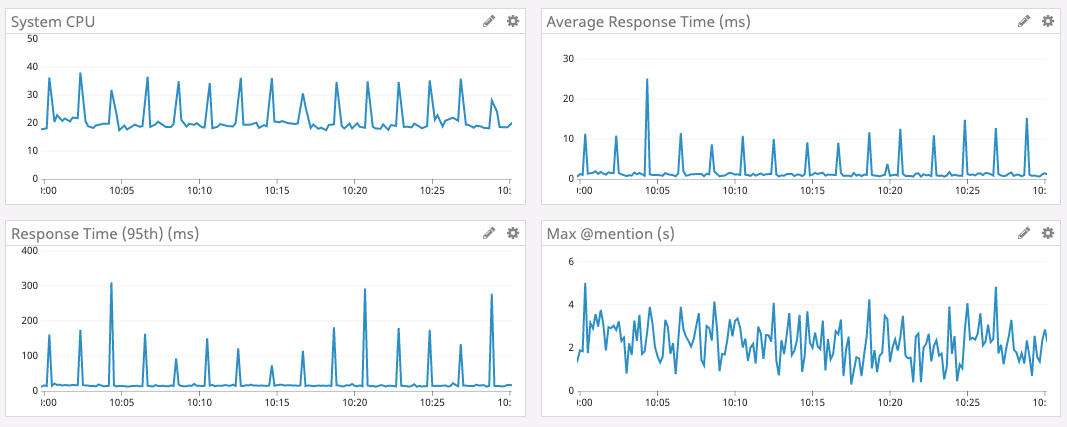
\includegraphics[width=0.8\textwidth]{images/golang-gc.png}
\end{center}

Quick recap: the Go garbage collector does its work and it adds a big latency spike. Rust would not have those spikes, because of ownership: when memory is no longer needed, it is trashed immediately and there's no waiting for the garbage collector to come by and decide if it can be cleaned up. To be fair, C++ also wouldn't have such spikes (because RAII). The article also adds that even with basic optimization, the Rust version performed better than the Go version. Not only in terms of there being no spikes, but in many dimensions: latency, CPU, and memory usage.

See the following graphs that compare Rust (blue) to Go (purple): 
\begin{center}
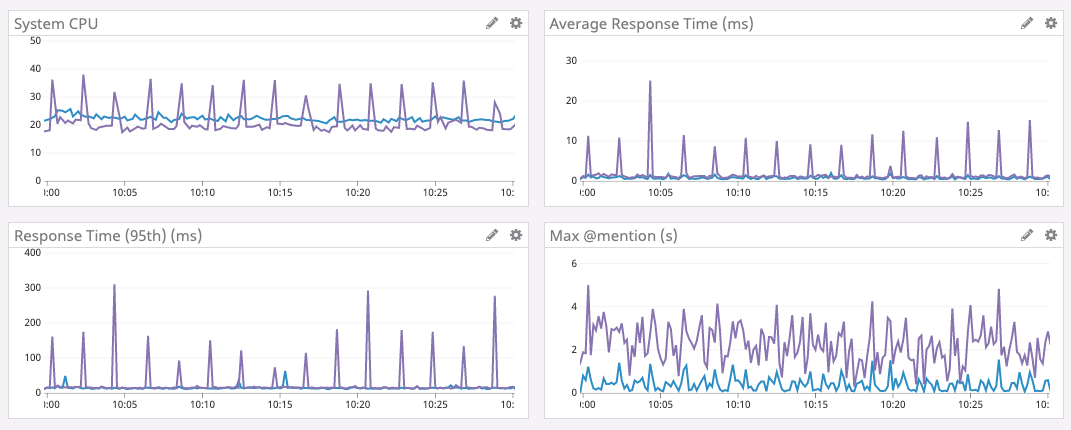
\includegraphics[width=0.8\textwidth]{images/rust-vs-go.png}
\end{center}

I do recommend reading the article because it goes into some more details and may answer some questions that you have. 

\paragraph{The Rules.}
That long introduction to the concept of ownership didn't explain very much about how it actually works; it just went into the \textit{why} and how it relates to the objectives of this course. But the rules are pretty simple---deceptively so---and they are as follows:

\begin{enumerate}
	\item Every value has a variable that is its owner.
	\item There can be only one owner at a time.
	\item When the owner goes out of scope, the value is dropped.
\end{enumerate}

These rules draw a distinction between the value itself and the variable that owns it. So in a statement of \texttt{let x = 42;} there is memory associated with the value "42". That memory is the "value" in rule 1, and its owner is the variable \texttt{x}.

When \texttt{x} goes out of scope, then the memory will be deallocated (``dropped''). (This is very much like the RAII (Resource Acquisition Is Initialization) pattern in languages like \CPP). Variable scope rules look like scope rules in other C-like languages. We won't belabour the point by talking too much about scope rules. But keep in mind that they are rigidly enforced by the compiler. See a brief example:
\begin{lstlisting}[language=Rust]
  fn foo() {
    println!("start");
    { // s does not exist
      let s = "Hello World!";
      println!("{}", s);
    } // s goes out of scope and is dropped
  }
\end{lstlisting}

The same principle applies in terms of heap allocated memory (yes, in Rust you cannot just pretend there's no difference between stack and heap, but ownership helps reduce the amount of mental energy you need to devote to this). Let's learn how to work with those! The example we will use is \texttt{String} which is the heap allocated type and not a string literal. We create it using the 
\begin{lstlisting}[language=Rust]
  fn main() {
    let s1 = String::from("hello");
    println!("s1 = {}", s1);
  }
\end{lstlisting}

A string has a stack part (left) and a heap part (right) that look like~\cite{rustdocs}:
\begin{center}
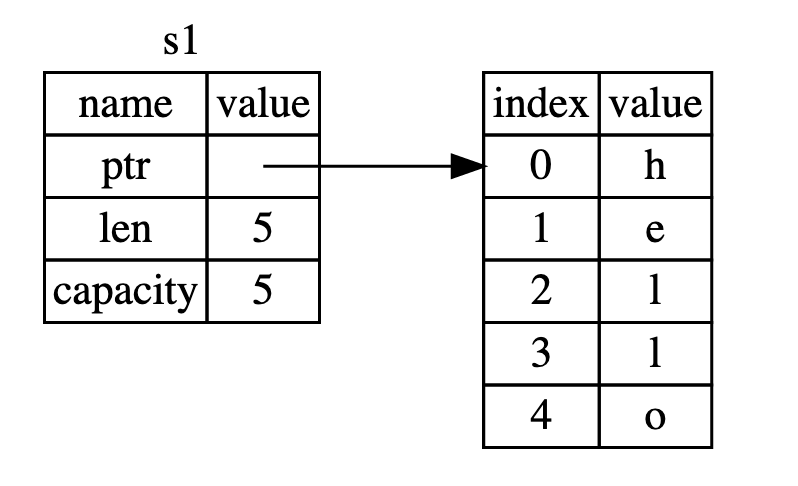
\includegraphics[width=0.33\textwidth]{images/string.png} 
\end{center}

This makes it a bit clearer about what is meant when the rules say that when the owner (the stack part) goes out of scope, the value (the heap part) is deallocated.

That covers rules one and three\ldots But that second rule is interesting, because of the ``at a time'' at the end: it means that there exists the concept of transfer of ownership.

In fact, everything we've said so far could also be true for much \CPP~code using RAII: there is an owner for each value, there is only one owner, and things are freed when they go out of scope. However, ``there is only one owner'' isn't actually enforced by the \CPP~compiler, so you can write code that breaks it, and then that code is prone to segfaults. 

\paragraph{What's yours is mine.}
Move semantics have to do with transferring ownership from one variable to another. But ownership is overkill for simple types\footnote{Specifically, types with the \texttt{Copy} trait have copy semantics by default; this trait is mutually exclusive with the \texttt{Drop} trait. \texttt{Copy} types have known size at compile time and can be stack-allocated.} (see the docs for a list---stuff like integers and booleans and floating point types), and such types don't need to follow move semantics; they follow copy semantics. Copy semantics are great when copies are cheap and moving would be cumbersome. So the following code creates two integers and they both have the same value (5).

\begin{lstlisting}[language=Rust]
  fn main() {
   	let x = 5;
	let y = x;
  }
\end{lstlisting}

But simple types are the exception and not the rule. Let's look at what happens with types with a heap component:

\begin{lstlisting}[language=Rust]
  fn main() {
    let s1 = String::from("hello");
    let s2 = s1;
  }
\end{lstlisting}

Here, no copy is created. For performance reasons, Rust won't automatically create a copy if you don't ask explicitly. (You ask explicitly by calling \texttt{clone()}). Cloning an object can be very expensive since it involves an arbitrary amount of memory allocation and data copying. This point is a thing that students frequently get wrong in ECE~252 in that that when doing a pointer assignment like \texttt{ thing* p = (thing*) ptr;} that no new heap memory was allocated and we have \texttt{p} and \texttt{ptr} pointing to the same thing. But that's not what happens in Rust~\cite{rustdocs}:

\begin{center}
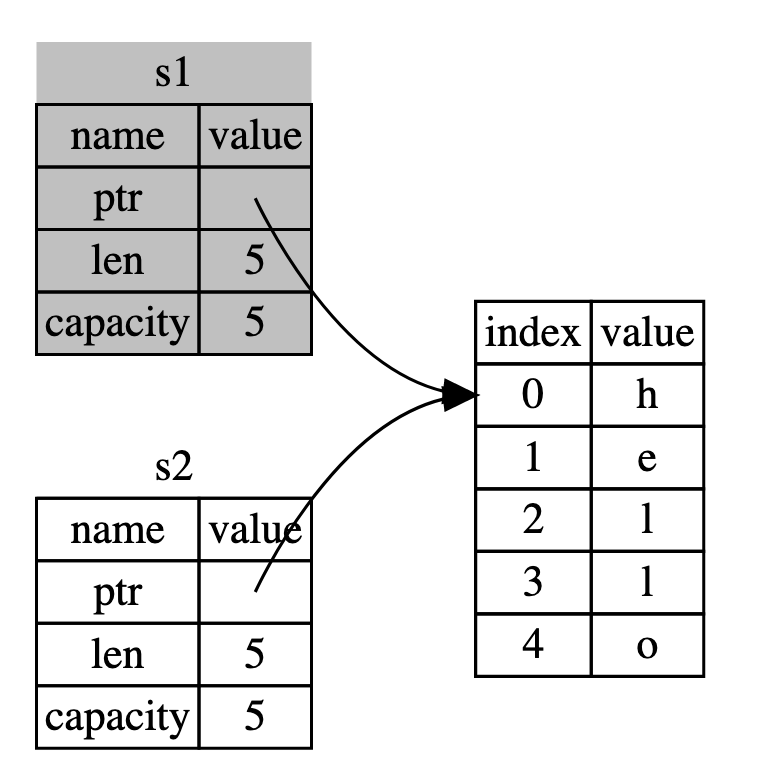
\includegraphics[width=0.3\textwidth]{images/string-rust.png}
\end{center}

If both \texttt{s1} and \texttt{s2} were pointing to the same heap memory, it would violate the second rule of ownership: there can be only one! So when the assignment statement happens of \texttt{let s2 = s1;} that transfers ownership of the heap memory to \texttt{s2} and then \texttt{s1} is no longer valid. There's no error yet, but an attempt to use \texttt{s1} will result in a compile-time error. Let's see what happens.

\begin{lstlisting}[language=Rust]
  fn main() {
    let x = 5;
    let y = x;
    dbg!(x, y); // Works as you would expect!

    let x = Vec<u32>::new(); // similar to the std::vector type in C++
    let y = x;
    dbg!(x, y); // x has been moved, this is a compiler error!
  }
\end{lstlisting}

The compiler is even kind enough to tell you what went wrong and why (and is super helpful in this regard compared to many other compilers)~\cite{rustdocs}:
\begin{verbatim}
plam@amqui ~/c/p/l/l/L02> cargo run
   Compiling move v0.1.0 (/home/plam/courses/p4p/lectures/live-coding/L02)
error[E0382]: use of moved value: `x`
 --> src/main.rs:8:10
  |
6 |     let x = Vec::<u32>::new(); // similar to the std::vector type in C++
  |         - move occurs because `x` has type `std::vec::Vec<u32>`, which does 
              not implement the `Copy` trait
7 |     let y = x;
  |             - value moved here
8 |     dbg!(x, y); // x has been moved, this is a compiler error!
  |          ^ value used here after move

error: aborting due to previous error

For more information about this error, try `rustc --explain E0382`.
error: could not compile `move`.

To learn more, run the command again with --verbose.
\end{verbatim}

Move semantics also make sense when returning a value from a function. In the example below, the heap memory that's allocated in the \texttt{make\_string} function still exists after the reference \texttt{s} has gone out of scope because ownership is transferred by the \texttt{return} statement to the variable \texttt{s1} in \texttt{main}.

\begin{lstlisting}[language=Rust]
  fn make_string() -> String {
    let s = String::from("hello");
    return s;
  }

  fn main() {
    let s1 = make_string();
    println!("{}", s1);
  }
\end{lstlisting}

This works in the other direction, too: passing a variable as an argument to a function results in either a move or a copy (depending on the type). You can have them back when you're done only if the function in question explicitly returns it! 

\begin{lstlisting}[language=Rust]
  fn main() {
    let s1 = String::from("world");
	use_string( s1 ); // Transfers ownership to the function being called
	// Can't use s1 anymore!
  }
  
fn use_string(s: String) {
    println!("{}", s); 
    // String is no longer in scope - dropped
}
\end{lstlisting}

This example is easy to fix because we can just add a return type to the function and then return the value so it goes back to the calling function. Great, but what if the function takes multiple arguments that we want back? We can \texttt{clone()} them all\ldots which kind of sucks. We can put them together in a package (structure/class/tuple) and return that. Or, we can let the function borrow it rather than take it\ldots But that's for next time!

\CPP~does have move semantics, but it uses copy semantics by default.

\paragraph{Do the Rules Work?}
With a stronger understanding of the rules and their practicalities, the obvious question is: do they work\textinterrobang There's no point in having the rules if they don't accomplish the goal. We'll assume for the moment that there are no bugs in the compiler that violate the expected behaviour. And then let's consider this from the perspective of some things that can go wrong in a C program.

(Okay, alright, before we get there---we'll eventually learn to break rules and to use reference counted objects where if we get it wrong we can leak. We briefly discuss \texttt{Rc} and \texttt{Arc} in Lecture 4.)

\begin{itemize}
	\item Memory leak (fail to deallocate memory)---does not happen in Rust because the memory will always be deallocated when its owner goes out of scope.
	\item Double-free---does not happen in Rust because deallocation happens when the owner goes out of scope and there can only be one owner.
	\item Use-after-free---does not happen in Rust because a reference that is no longer valid results in a compile time error.
	\item Accessing uninitialized memory---caught by the compiler.
	\item Stack values going out of scope when a function ends---the compiler will require this be moved or copied before it goes out of scope if it is still needed.
\end{itemize}

\subsection*{A free lunch?}
To provide a somewhat balanced view, Rust of course doesn't solve every problem
in the world. It does solve memory management well, and I wouldn't even say that
it requires more of the programmer: it requires more of the programmer at compile-time,
not at debug-time.

Here are some downsides to consider:
\begin{itemize}
\item Static typing: To expand on the point above: there is a New Zealand saying ``she'll be right''. It's a bit hard to explain, but Wikipedia suggests: ``a situation or object which is not perfect but is good enough to fulfil its purpose''. Static typing, and Rust, discourage this point of view. The code really does have to satisfy type safety and memory safety properties before it will run.
\item Ecosystem: Rust does come with a package registry (crates), which is better than \CPP, but some libraries are not going to exist in Rust. We'll talk more about calling foreign functions in Lecture 5.
\item Compiler: Rust's compiler can be slow on large codebases.
\end{itemize}

For additional balance, let's revisit garbage collection. If you want
to implement graphs and doubly-linked lists\footnote{\url{https://rust-unofficial.github.io/too-many-lists/}}, GC is really handy. (Many
Rust people will argue that you shouldn't use linked lists if you want
performance anyway. If you think back to your architecture course, you
can deduce why.) Or you can use pointers and unsafe Rust and hope to
get it right.

\bibliographystyle{alphaurl}
\bibliography{459}


\end{document}
